\chapter{Abstract}
\label{ch:Abstract}

With the ever increasing amount of data to be rendered for a single given scene, experimenting with new approaches for handling and structuring that data becomes more and more important. This paper covers the approach to enhance response times and quality using out-of-core techniques. \\

With the help of out-of-core techniques, it is possible to achieve real-time rendering performance on current-generation graphics cards by overcoming limits posed by the graphics cards' internal memory \cite{Crassin:2009:GRS:1507149.1507152}. Thus, this topic is essential for everyone hoping to achieve such performance for scenes that cannot be efficiently rendered using conventional methods. \\

I will discuss different strategies used to load necessary data chunks into working memory taking into account its finiteness using intelligent data streaming. These include visibility culling and virtual texturing. Also, this paper will give an overview of the possibility to use volumetric texture units called ``Voxels'' instead of regular texels and the advantages and challenges that come with it. Lastly, the topic will be further explored using the examples \cite{Crassin:2009:GRS:1507149.1507152} and \cite{van2009id}.

\chapter{Motivation}
\label{ch:Motivation}

Over the course of the last years, the complexity of scenes to be rendered has risen further and further. Nowadays, performance and complexity demands cannot be satisfied by solely utilizing brute force methods and trying to fit all necessary data into the scarce graphics memory. There are a number of specific use cases where another approach is needed. For example, \cite{10.1007/978-3-540-40014-1_3} look for a way to interactively render very large landscapes in the context of virtual reality using commmodity graphics hardware. Further, \cite{Gobbetti:2005:FVM:1073204.1073277} name the fields of 3D scanning, computer-aided design and numerical simulation.

In essence, all of these use cases require a technique able to expand available memory by making use of larger but slower storage. While doing this, the searched technique should also minimize response times which are bound to increase due to longer memory access times. A technique that finds a suitable compromise between memory extension and response times is called an Out-of-Core technique.

\chapter{Basics}
\label{ch:Basics}

This chapter aims to introduce key terminology that will be used in this paper. The chapter gives a basic understanding of the terms ``Texture Mapping'', ``Memory Virtualization'', ``Virtual Texture'' and ``Level of Detail''.

\section{Texture Mapping}

Texture mapping provides a way of adding detail to rendered surfaces without increasing geometric complexity. In its simplest form, it takes a 2-dimensional image called \textit{texture map} and a 3-dimensional model and paints the image onto the model. \textit{Texture coordinates} are used to determine which point on the texture map corresponds to a point on the model.

\begin{figure}[h]
  \begin{center}
    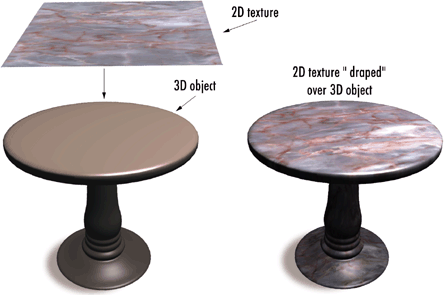
\includegraphics[width=.3\textwidth]{logos/texture_mapping_example.png}
    \hfill
    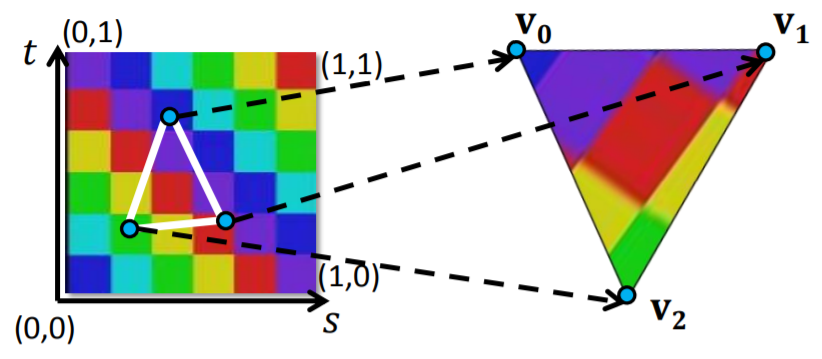
\includegraphics[width=.5\textwidth]{logos/texture_coordinates_example.png}
    \caption{A texture is mapped onto the table model, making it more realistic. Images from \cite{TextMapExample} and \cite{CompGraphics:2017:04:TexMap}}
  \end{center}
\end{figure}

The first notable paper about texture mapping was published by \cite{catmull1974subdivision} in 1974. After that, texture mapping became particularly popular in video games of the 90's and is now a crucial part of the vast majority of computer-rendered scenes. Because of its usefulness, the concept of texture mapping was extended from affecting the diffuseness to also altering other aspects like specularity, lighting and normals.

\section{Memory Virtualization}

Memory virtualization is the process of abstracting from the physical memory available. The initial motivation for this concept was to enable the uniform usage of heterogeneous storage devices \cite{Euler:VirtualMemoryHistory:2008}. However, it also has more advantages. Firstly, memory fragmentation is reduced, decreasing average memory access times. Secondly, virtual memory can combine (graphics) main memory and slower storage and thus increase the total space available to load data into. Other aspects of memory virtualization are beyond the scope of this paper. The most important aspect of memory virtualization regarding rendering large amounts of data is its ability to extend available memory as this solves one of the issues mentioned in \ref{ch:Motivation}.

The Windows Display Driver Model v2.0 supports graphics memory virtualization under Windows 10 \cite{Microsoft:GPUVirtualMemory:2017}. However, page faults cause rendering to halt until the requested page is loaded. This makes this solution unsuitable on its own as it reduces responsiveness.

\section{Virtual Texture}

A virtual texture is, in general, a texture too large to fit into the physical graphics memory that is available in virtual memory. 

\begin{figure}[h]
  \begin{center}
    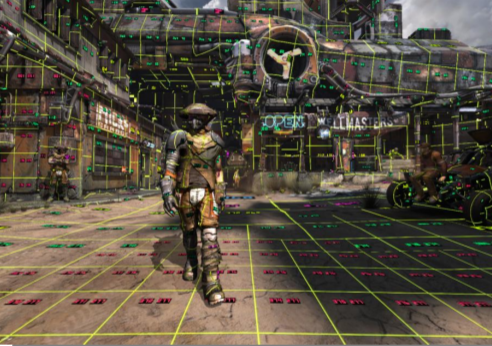
\includegraphics[width=.3\textwidth]{logos/virtual_texture_example.png}
    \caption{Image only shows a tiny portion of the actual virtual texture. Different levels of detail can be seen. Image from \cite{van2009id}}
  \end{center}
\end{figure}

The advantage of a virtual texture over a conventional physical texture is its ability to hold significantly larger amounts of rendering data. For example, id Tech 5 uses virtual textures that consist of approximately 16.3 billion texels \cite{van2009id}. Without special handling, virtual textures face the same responsiveness issues as virtual memory.

\section{Level of Detail}

Level of Detail refers to altering an object's complexity between rendered frames. An example of this technique applied to textures is mip-mapping. 

\begin{figure}[h]
  \begin{center}
    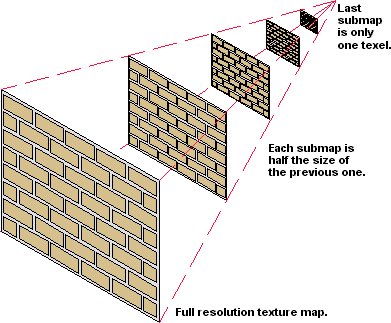
\includegraphics[width=.3\textwidth]{logos/mipmap_example.png}
    \caption{A texture is saved at different resolutions. As the viewer moves closer, resolution is increased and vice versa. Image from \cite{PCMag:DefMipMapping:2017}}
  \end{center}
\end{figure}

Level of Detail addresses the issue of increasing scene complexity as the viewpoint moves away from a limited clip and its environment moves into view. Decreasing the complexity of the objects furthest away from the camera increases rendering performance while not significantly affecting quality \cite{Unity:LevelOfDetail:2017}. Hence, Level of Detail can be used to address the aspect of responsiveness mentioned in \ref{ch:Motivation}.

\chapter{Main Content}
\label{ch:MainContent}

\section{Memory Management}
%% ==============
Here I will talk about ways to utilize slow external memory to be able to store large datasets without losing wanted performance. I will refer to voxels, virtual paging and other techniques.

\section{Voxels}

Here I will give a detailed overview of the concept of voxels. I will talk about their differences to texels, advantages, challenges and their suitability for out of core processes.

\section{Example 1: GigaVoxels}
%% ==============
Here I will use the discussed concepts to explain how GigaVoxels can be used to render large volumetric datasets with high performance. I will explain how this is related to both voxels and out of core processes.

\section{Example 2: ID Tech 5 Challenges}
Here I will discuss in detail how out of core rendering is compatible with parallelization using the ID Tech 5 Challenges example. I will talk about the faced challenges and how they were solved. 

\section{Example 3: Visualization of very large Landscapes}
Here I will summarize the findings from \cite{10.1007/978-3-540-40014-1_3}. I will refer to multi-resolution algorithms and how they are related to the topic.

\chapter{Epilogue}
\label{ch:Epilogue}

Here I will outline how out of core techniques can be used to develop new ways of data provision and rendering scenes in the future. 